\chapter{Evaluation}
\label{chap:evaluation}

% All numbers are measured; raw data and scripts: scripts/eval/ and
% scripts/eval/out/ in the repository (summary.csv is the machine index).
% Live measurements: ARES, 8-node ChronoLog deployments, 2026-07-30/31.

The evaluation asks six questions, mapped to the requirements of
\S\ref{sec:problem-requirements}: what does capture cost the observed
workload (R5, \S\ref{sec:eval-overhead}); how fresh are the live views
(R2, \S\ref{sec:eval-freshness}); is the Doctor's diagnosis
\emph{correct}, not merely cheap (R6, \S\ref{sec:eval-doctor}); do the
analyses scale as claimed (R4,
\S\ref{sec:eval-scalability}); does the whole stack work end-to-end on a
real cluster with real agents (R1, R3, R7,
\S\ref{sec:eval-functional}); and does the system actually shorten the
path from symptom to cause (\S\ref{sec:eval-casestudy}).
Section~\ref{sec:eval-limitations} discusses limitations.
Table~\ref{tab:eval-glance} previews the headline results.

\begin{table}[t]
\centering
\small
\begin{tabular}{@{}p{0.34\linewidth}p{0.58\linewidth}@{}}
\toprule
\textbf{Question} & \textbf{Measured answer} \\
\midrule
What does capture cost the agent? &
  It adds $3.6$\,ms to a turn that averages $7.7$\,seconds, under
  $0.05\%$. Run against real agents with capture on and off, the
  difference was too small to measure (\S\ref{sec:eval-overhead}). \\
How fresh are the live views? &
  An event reaches the operator's screen in $10.7$\,ms. The durable
  archive takes $20$--$30$\,s to catch up, so the live view is roughly
  $1\,900\times$ faster (\S\ref{sec:eval-freshness}). \\
Is the diagnosis correct? &
  It found all $580$ planted faults and raised no false alarms on clean
  data. Five hundred identical errors were presented as one ranked
  incident (\S\ref{sec:eval-doctor}). \\
Do the analyses scale? &
  Fleet queries stayed at $19$--$24$\,ms while stored events grew
  $50\times$, and grow linearly with fleet size: $49$\,ms at 400 nodes
  of synthetic state (\S\ref{sec:eval-scalability}). \\
Does it run for real? &
  The whole stack passed all $28$ end-to-end checks on live 4- and
  8-node clusters, running up to $32$ real agents without per-node cost
  rising (\S\ref{sec:eval-functional}, \S\ref{sec:eval-scalability}). \\
Does it shorten diagnosis? &
  An operator meeting the fault for the first time diagnosed it
  completely in $72$\,seconds. From the raw logs the same operator could
  not answer any of the three questions (\S\ref{sec:eval-casestudy}). \\
\bottomrule
\end{tabular}
\caption[The evaluation at a glance]{The evaluation at a glance. Every number is measured; the
sections referenced give conditions, distributions, and caveats.}
\label{tab:eval-glance}
\end{table}

\section{Methodology}
\label{sec:eval-method}

\paragraph{Platform.} All live experiments run on the ARES cluster under
SLURM. Each experiment allocates $M$ idle compute nodes and deploys
ChronoLog across them (visor, one keeper per node, grapher draining to
an archive on shared storage), followed by the observability components:
one collector and one capture-worker process per node, and one dashboard
on a designated node. The deployments evaluated live use $M = 4$ and
$M = 8$. In this configuration the keeper seals 10\,s story chunks under a
15\,s acceptance window, while the grapher and player run with a
180\,s acceptance window; \S\ref{sec:eval-freshness} measures what these
settings translate to end-to-end, and corrects a folklore number in the
process.

\paragraph{Workloads.} Two workloads exercise the identical ingest path.
\emph{Real agents}: Claude Agent SDK agents, one or more per node
(configurable as $K$ agents per node), each performing genuine LLM turns
and one cross-node delegation through a remote-agent MCP tool per
round; turns enter Path-A, edges Path-B. \emph{Synthetic traffic}: a
generator that emits realistic interaction records and
\texttt{start}/\texttt{done} edge pairs through the same spool and
collector endpoints, with configurable topology (mesh, star, pipeline,
ring), agent count, node spread, error rate, and pacing. Real agents
provide ground truth end-to-end; synthetic traffic provides controlled,
reproducible, zero-token-cost load for overhead and scalability
measurements, and is the fault-injection vehicle for
\S\ref{sec:eval-casestudy}.

\paragraph{Measurements.} Latency overhead is measured as the difference
in per-turn wall-clock between instrumented and uninstrumented runs of
the same agent workload; capture-side costs by sampling the sidecar
processes' CPU and resident memory under load; storage by bytes per
record in each tier; freshness by timestamping an event at emission and
at receipt in a subscribed SSE client. Each is reported with distribution
statistics over repeated runs rather than as a single number: the workload
under test is a non-deterministic one running on shared cluster hardware,
which is exactly the regime in which single-run comparisons are known to
mislead, and in which a difference must be stated with a confidence
interval or not stated at all~\cite{georges2007rigorous}. Percentiles
rather than means are reported wherever an operator's experience is
governed by the tail~\cite{dean2013tail}.

\section{Capture Overhead}
\label{sec:eval-overhead}

Capture overhead is the cost the observed workload pays, and the design
predicts it is small by construction: the Path-A fast path is one local
JSONL append (no network, no lock, no downstream dependency,
\S\ref{sec:design-write}); the Path-B fast path is one HTTP POST to a
daemon on \texttt{localhost} that enqueues and returns. Both are
constant-time and independent of history size. Everything else (the
ChronoLog write, the forward, the drain) happens in sidecar processes
off the agent's critical path.

Figure~\ref{fig:capture-overhead} shows what capture adds to each event on
the agent's critical path, and Table~\ref{tab:overhead} the standing
resource and storage costs that a latency plot cannot show. All latency
numbers are taken on live compute nodes with the production NFS state
directory: the real deployment condition, not a tmpfs microbenchmark.

\begin{figure}[h]
  \centering
  % Capture overhead per event, by path (E1a/E1b; see tab:overhead for the
% resource and size rows). \input this inside a figure environment;
% needs \usepackage{pgfplots}.
%
% Data: scripts/eval/out/e1a_spool_latency_compute.csv (spool),
%       e1b_emit_collector.csv (collector), e1b_emit_fallback.csv (fallback);
% p50/p95 recomputed from those files and cross-checked against results.md.
%
% NOTE: the category names are used directly as the symbolic y coordinates.
% Do NOT reintroduce a separate `yticklabels={...}` list: with `ytick=data`
% pgfplots orders ticks by their order of appearance in the coordinate list,
% not by the `symbolic y coords` declaration, so a separate label list
% silently attaches the wrong name to each bar.
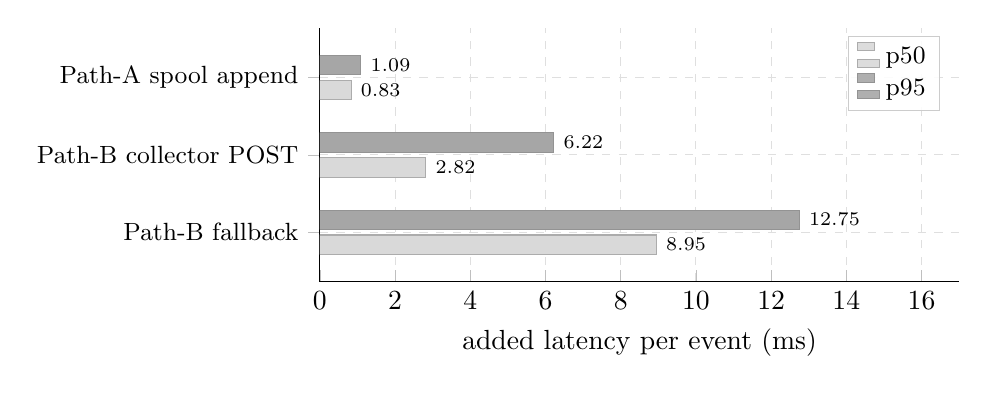
\begin{tikzpicture}
\begin{axis}[
    width=0.80\linewidth, height=4.8cm,
    xbar, bar width=7pt,
    xlabel={added latency per event (ms)},
    xmin=0, xmax=17,
    symbolic y coords={{Path-B fallback},{Path-B collector POST},{Path-A spool append}},
    ytick=data,
    yticklabel style={font=\small},
    nodes near coords, nodes near coords align={horizontal},
    every node near coord/.append style={font=\scriptsize, text=black},
    legend pos=north east, legend cell align=left,
    legend style={font=\small, draw=gray!40, fill=white, fill opacity=0.9,
                  text opacity=1},
    grid=major, grid style={dashed,gray!25},
    enlarge y limits=0.32,
    axis lines*=left,
    tick style={draw=gray!50},
]
\addplot[fill=gray!30, draw=gray!65, mark=none] coordinates {
    (0.83,{Path-A spool append})
    (2.82,{Path-B collector POST})
    (8.95,{Path-B fallback})};
\addplot[fill=gray!70, draw=gray!85, mark=none] coordinates {
    (1.09,{Path-A spool append})
    (6.22,{Path-B collector POST})
    (12.75,{Path-B fallback})};
\legend{p50, p95}
\end{axis}
\end{tikzpicture}

  \caption[Capture overhead per event, by path]{What capture adds to the
  agent's critical path, per event ($n{=}10\,000$ per bar, live 8-node
  deployment, production NFS state directory). Path-A's spool append is a
  local file write and costs under a millisecond. Path-B's POST to the
  node-local collector costs a few. The bottom pair is the degraded mode
  taken when the collector is down: the agent posts directly to the
  dashboard, at roughly $3\times$ the cost. Degradation is slower, not
  cheaper, which is why the collector exists. For scale, the mean LLM turn
  these sit inside is $7\,734$\,ms, three orders of magnitude to the right
  of this axis.}
  \label{fig:capture-overhead}
\end{figure}

\begin{table}[h]
\centering
\small
\begin{tabular}{@{}lllr@{}}
\toprule
\textbf{Cost} & \textbf{Path} & \textbf{Metric} & \textbf{Measured} \\
\midrule
\textbf{End-to-end turn delta} & A{+}B & instrumented vs.\ not, per turn &
  \textbf{$+365 \pm 2\,398$\,ms} \\
Collector daemon      & B & CPU / RSS per node, 20\,ev/s     & 32\% / 40\,MB \\
Capture worker        & A & CPU / RSS per node, same load    & 0.8\% / 51\,MB \\
Interaction record    & A & bytes per event (spool / archive) & 2\,093 / 2\,173\,B \\
Edge event            & B & bytes per event (hot / archive)   & 612 / ${\approx}560$\,B \\
Live forward          & B & bytes per event on the wire       & 646\,B \\
\bottomrule
\end{tabular}
\caption[Capture overhead: standing costs]{The standing costs of capture,
alongside the per-event latencies of Figure~\ref{fig:capture-overhead}
(live 8-node deployment, compute nodes, NFS state directory).
The first row is the end-to-end A/B turn delta over real LLM turns:
its 95\% confidence interval spans zero, so capture is statistically
invisible inside the workload's own variance. Capture worker CPU is the
mean of a bursty profile (idle between 5\,s drain passes, peaks of 85\%
during them); the wire number is amortized over batches of ${\le}64$
(658\,B unbatched).}
\label{tab:overhead}
\end{table}

The headline is easy to over- and under-claim, so it needs stating
carefully. The A/B experiment ran $n{=}30{+}30$ real agent turns
(identical prompts, interleaved to absorb provider drift): instrumented
turns averaged $8\,099 \pm 5\,147$\,ms, uninstrumented
$7\,734 \pm 4\,291$\,ms, a delta of $+365$\,ms whose 95\% confidence
interval ($\pm 2\,398$\,ms, Welch $t = 0.30$) makes it statistically
indistinguishable from zero. The claim therefore rests on both
measurements: the \emph{mechanism} costs
$0.83 + 2.82 \approx 3.6$\,ms per turn-plus-delegation (under
\textbf{0.05\%} of a 7.7\,s mean turn), and the A/B run confirms that
nothing beyond the mechanism leaks onto the critical path. With the
collector \emph{down}, the fallback POST to the dashboard costs
$3\times$ the normal path (8.95 vs.\ 2.82\,ms p50): degraded mode is
slower, not cheaper, which is why the collector exists.

Two structural observations frame the numbers. First, the denominator is
large: an LLM turn takes seconds and a delegation round-trip longer, so
capture cost in milliseconds translates to a per-turn overhead orders of
magnitude below the workload's own variance. This is the inverse of the
classical tracing regime (\S\ref{sec:bg-sampling}), where sub-millisecond
RPCs made even microseconds of instrumentation significant; it is
why complete capture is affordable here. Second, the failure-mode cost is
bounded by design rather than measured luck: if every downstream component
dies, the agent's cost is unchanged (Path-A) or one failed local
connection followed by a fallback POST (Path-B).

\section{Freshness and Query Latency}
\label{sec:eval-freshness}

Freshness is the interval from an agent emitting an event to that event
being visible to an operator. The claim under test is that the hot path
(R2) puts the event on screen in milliseconds while the cold path
delivers durability in tens of seconds, and the measurement corrects a
number this thesis itself repeated from deployment folklore.

Figure~\ref{fig:query-latency} plots the whole range on one axis: the
hot-path pipeline (emit $\to$ collector $\to$ dashboard ingest $\to$ SSE
frame at a subscribed client), each per-view query against the populated
live deployment, and the cold-path drain they must all be read against.
Four numbers do not fit on that axis and are given in
Table~\ref{tab:freshness}: the tails, the degraded path, and the
rollup-backed fleet read that \S\ref{sec:eval-scalability} explains.

\begin{table}[h]
\centering
\small
\begin{tabular}{@{}llr@{}}
\toprule
\textbf{Measure} & & \textbf{Measured} \\
\midrule
Emit $\to$ SSE frame at client   & p95          & 11.8\,ms \\
\quad direct-ingest fallback     & p50 / p95    & 8.5 / 8.9\,ms \\
Cold-path availability (drain)   & max, $n{=}10$ & 30\,s \\
Fleet health, rollup-backed (\S\ref{sec:eval-scalability}) & p50 & 19--24\,ms \\
\bottomrule
\end{tabular}
\caption[Freshness and query latency: tails and degraded paths]{The
freshness numbers Figure~\ref{fig:query-latency} cannot show: the tail of
the live push, the degraded direct-ingest path taken when the collector is
down, the worst drain observed, and the rollup-backed fleet read.
Live 8-node deployment, dashboard node, $n{=}100$ per query row,
$n{=}1\,000$ paced events at 20\,ev/s with zero loss for the SSE rows,
corpus ${\approx}22$\,k archived events.}
\label{tab:freshness}
\end{table}

\begin{figure}[t]
  \centering
  % Freshness / query latency spread, one log axis (p50, live 8-node run).
% Data: scripts/eval/out/summary.csv (E2a live, E2c live rows).
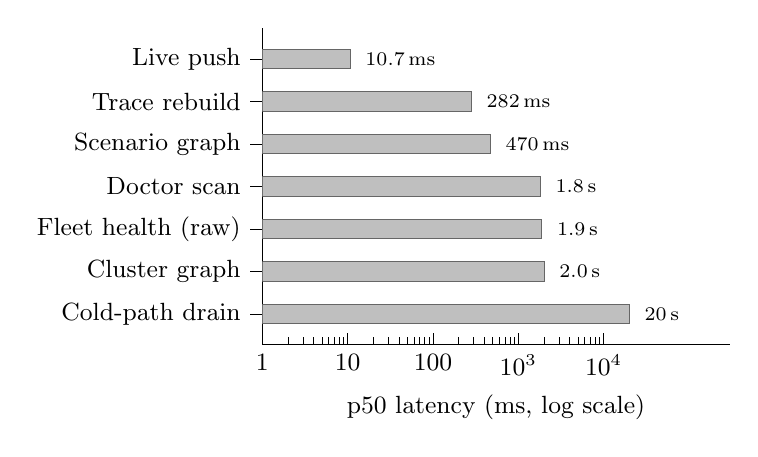
\begin{tikzpicture}
\begin{axis}[
    xbar,
    xmode=log,
    log origin=infty,
    width=0.62\linewidth,
    height=5.6cm,
    xmin=1, xmax=300000,
    xtick={1,10,100,1000,10000},
    xticklabels={1,10,100,$10^3$,$10^4$},
    xlabel={p50 latency (ms, log scale)},
    symbolic y coords={
      {Cold-path drain},
      {Cluster graph},
      {Fleet health (raw)},
      {Doctor scan},
      {Scenario graph},
      {Trace rebuild},
      {Live push}},
    ytick=data,
    y dir=normal,
    yticklabel style={font=\small},
    xticklabel style={font=\small},
    xlabel style={font=\small},
    nodes near coords,
    nodes near coords style={
      font=\scriptsize, anchor=west, xshift=2pt},
    point meta=explicit symbolic,
    bar width=7pt,
    enlarge y limits=0.12,
    axis lines*=left,
    tick style={black},
]
\addplot[fill=black!25, draw=black!60] coordinates {
  (10.7,{Live push}) [10.7\,ms]
  (282,{Trace rebuild}) [282\,ms]
  (470,{Scenario graph}) [470\,ms]
  (1807,{Doctor scan}) [1.8\,s]
  (1881,{Fleet health (raw)}) [1.9\,s]
  (2009,{Cluster graph}) [2.0\,s]
  (20000,{Cold-path drain}) [20\,s]
};
\end{axis}
\end{tikzpicture}

  \caption[Freshness and query latency, measured]{The freshness and query-latency spread on one log axis (p50,
  live 8-node deployment). Live push takes single-digit milliseconds and
  scenario-scoped reads stay sub-second, while population-wide reads
  that fold the raw archive sit near $2$\,s on this corpus. That is the
  linear-in-events cost the rollup design of
  \S\ref{sec:eval-scalability} flattens to roughly $20$\,ms.}
  \label{fig:query-latency}
\end{figure}

\paragraph{The drain is 20--30\,s; the ``$\sim$180\,s'' was something
else.} Measured directly (append a marked event, poll the archive), a
story chunk becomes readable \textbf{20--30\,s} after append ($n{=}10$,
p50 20\,s), governed by the keeper's 10\,s chunking and 15\,s
acceptance window plus the grapher's write batch, not by the 180\,s
window configured downstream. The ${\sim}180$\,s that operators (and
earlier drafts of this thesis) attributed to the drain is in fact the
client's \emph{replay-query timeout}. In these deployments the player's
playback responses never reach the dashboard process's receiver
service: the player logs every request and completes none of the
transfers toward that endpoint, while an otherwise-identical receiver
in the capture process works. Every live replay issued by the dashboard
therefore blocks for the full \texttt{CL\_ERR\_QUERY\_TIMED\_OUT}
window of ${\sim}180$\,s: per story, per request, holding the client
lock.
Diagnosing this (\S\ref{sec:eval-limitations}) explained the
folklore number and motivated generalizing the archive-first read rule
of \S\ref{sec:design-read} from listing indexes to \emph{all} dashboard
replays: with the drain at 20--30\,s, serving full-fidelity views from
the archive costs at most half a minute of staleness and removes the
last blocking read from the serving process.

Qualitatively, the split then behaves as designed in every live run: the
live views (scenarios, cluster, fleet, health, traces) render
immediately during a run, while full-fidelity conversation views fill in
within the half-minute drain; no view blocks the dashboard, fresh
clusters included.

\section{Detection Quality}
\label{sec:eval-doctor}

R6 demands that diagnosis be free of marginal token cost; this section
asks whether the deterministic pipeline that satisfies it is also
\emph{correct}. The experiment scores a full Doctor scan (gather,
detect, cluster, diagnose, record; \S\ref{sec:analytics-doctor})
against a ground-truth manifest of
injected faults. Deliberately injecting the failure and checking that the
system reports it is the discipline of controlled fault
injection~\cite{basiri2016chaos}, applied here offline rather than in
production so that the manifest is exact and the false-positive rate is
measurable against a known-clean background.
A controlled corpus is seeded offline through the same
spool and inter-agent-store write paths the capture layer uses: a clean
background of healthy traffic (216 turns, 120 completed delegations),
plus ten planted faults of each of the eight detector families of
\S\ref{sec:analytics-doctor} (5xx errors, rate-limiting, retry storms,
latency outliers, edge errors, orphan calls, slow edges, recoveries),
plus one \emph{storm} (500 identical peer-timeout edges spread across 40
hosts) to test that section's compression claim. Each planted fault is
shaped to carry exactly one symptom (single-label ground truth), so every
detection is unambiguously attributable. The same fault mix is then
injected a second time and the corpus re-scanned, testing whether the
incident history recognizes the recurrence.

The result is a clean sweep: all 580 planted signals were detected, the
eighty single faults and every event of the storm alike, and every
incident was routed to its intended diagnosis rule, at confidences from
0.55 (latency outliers, slow edges) to 0.85 (rate limiting). The scan is
seed-deterministic (\texttt{e6\_doctor\_\allowbreak quality.py} in
\texttt{scripts/eval/}), and the result is identical at $n{=}25$ and
under a different seed.

Three results carry the argument. First, the clean background
produces \emph{zero} incidents: the detectors' thresholds (medians with
absolute floors, consecutive-repeat minima) do not fire on healthy
variance, so a ranked incident list starts empty rather than requiring
the operator to learn a noise floor. Second, compression behaves as
designed: 580 injected raw signals become 9 ranked incident cards;
in particular the 500 identical timeouts collapse into \emph{one} card
whose count, host list, and severity escalation carry the blast radius
(the ``not a scroll of per-event errors'' the operator asked for). Third,
the longitudinal claim holds mechanically: after the first scan writes the incident
memory, the second scan badges all nine incidents as recurring with the
correct prior count, read back from the self-compacting memory document
rather than from process state.

The scope of the claim is bounded. The planted faults are
in-distribution and comfortably above the detector thresholds: the
experiment establishes that detection, clustering, diagnosis routing,
and cross-run memory are correct on unambiguous faults, not that the
thresholds are well-calibrated on borderline cases. ``Diagnosis
correct'' likewise means only that the incident reached the intended
rule of the hand-built rule set, whose coverage limits are discussed in
\S\ref{sec:eval-limitations}. A perfect score under these conditions is
the expected behavior of deterministic detectors, not evidence against
harder inputs; the informative results are the zero-false-positive
background, the exact $500{\to}1$ compression, and the memory
round-trip.

\section{Scalability}
\label{sec:eval-scalability}

The evaluation tests three scaling claims.

\paragraph{Fleet reads are independent of event volume.} The rollup
design (\S\ref{sec:analytics-fleet}) makes the fleet query
$O(\text{nodes} \times \text{buckets})$; the raw-fold fallback is
$O(\text{events})$. The experiment holds nodes and window fixed (16
nodes, 60-minute window) and grows the event count from $10^4$ to
$5 \times 10^5$, comparing the fleet-health query latency of the two
paths (20 requests per point, p50). Figure~\ref{fig:rollup-scaling}
shows the result: rollup-backed reads stay flat at 19--24\,ms across a
$50\times$ growth in event volume, while the raw fold grows linearly
(slope ${\approx}17$\,ms per thousand events between the endpoints):
107\,ms at 10\,k events, 8.5\,s at 500\,k, a $457\times$ gap at the
largest size.

\paragraph{Fleet reads grow linearly in fleet size, and only in fleet
size.} The complementary experiment holds the per-node event density fixed
and grows the \emph{number of nodes}. It cannot be run on the live
allocation: the largest cluster available here was eight nodes
(\S\ref{sec:eval-functional}). It is therefore run against
\emph{synthetic fleet state}: the harness invents $n$ host names and
writes their events through the production capture API, the production
emitter bucketizes them, and the production dashboard is then queried over
HTTP exactly as an operator would. What is synthetic is the origin of the
events; the store, the query path and the measured latency are the real
ones. This is sufficient for the claim under test, which is a property of
the read algorithm: the fold cost depends on how many buckets exist, not on
which machine produced them. It is correspondingly \emph{not} evidence
about capture, drain or network behaviour at that scale, which the live
4- and 8-node deployments cover instead.

Figure~\ref{fig:fleet-nodes} shows the result over fleets of 10 to 400
nodes (50 requests per point). Latency is linear in node count,
$5.2 + 0.105n$\,ms with $R^2 = 0.98$: a fixed ${\sim}5$\,ms of request
handling plus ${\sim}0.1$\,ms per node summarized. A 100-node fleet is
answered in 14.7\,ms p50 and a 400-node fleet in 49.0\,ms, both inside
interactive time, where the same query folded from raw events would touch
every record ever captured. The 100-node point reproduces an
independent measurement taken on the cluster three weeks earlier
(15.1\,ms), which is the reason to trust the rest of the curve. The sweep
stops at 400 nodes because that is the emitter's configured session bound
(\texttt{max\_sessions}, \S\ref{sec:analytics-fleet}); beyond it the
harness silently re-measures a 400-node fleet rather than a larger one.

\begin{figure}[t]
  \centering
  \input{figures/fig-rollup-scaling}
  \caption[Fleet-query latency vs.\ stored event count]{Fleet-health query latency vs.\ stored event count (16 nodes,
  60-minute window, p50 over 20 requests). Pre-aggregated rollup reads
  are independent of event volume; the raw-fold fallback is linear in
  it. Measured offline via
  \texttt{bench\_rollup\_\allowbreak scaling.py} in
  \texttt{scripts/eval/}.}
  \label{fig:rollup-scaling}
\end{figure}

\begin{figure}[t]
  \centering
  % Fleet-health query latency vs. FLEET SIZE (E3b, re-measured 2026-08-10).
% Complements fig-rollup-scaling, which holds nodes fixed and grows events.
% \input this inside a figure environment; needs \usepackage{pgfplots}.
%
% Data: thesis/figures/e3b_heatmap_nodes_p50.csv, derived from
% scripts/eval/out/e3b_heatmap_nodes.csv (50 requests per point, synthetic
% fleet state, real dashboard, ARES gateway).
\begin{tikzpicture}
\begin{axis}[
    width=0.85\linewidth, height=6cm,
    xlabel={fleet size (nodes; synthetic rollup state)},
    ylabel={\texttt{/api/fleet/health} latency (ms)},
    xmin=0, xmax=420, ymin=0,
    legend pos=north west, legend cell align=left,
    legend style={font=\small, draw=gray!40},
    grid=major, grid style={dashed,gray!25},
    tick style={draw=gray!50},
]
\addplot[dashed, gray!70, domain=0:400, samples=2] {5.20 + 0.1053*x};
\addlegendentry{$5.2 + 0.105\,n$ (fit, $R^2{=}0.98$)}
% Styles set explicitly rather than taken from the cycle: the dashed fit line
% above consumes a cycle index, which would otherwise render p95 heavier than
% p50 and make the secondary series the visually dominant one.
\addplot[black!80, thick, mark=*, mark size=1.6pt,
         mark options={fill=black!30, draw=black!80}]
    table [x=nodes, y=p50_ms, col sep=comma]
    {figures/e3b_heatmap_nodes_p50.csv};
\addlegendentry{p50}
\addplot[black!45, thick, mark=square*, mark size=1.6pt,
         mark options={fill=black!8, draw=black!45}]
    table [x=nodes, y=p95_ms, col sep=comma]
    {figures/e3b_heatmap_nodes_p50.csv};
\addlegendentry{p95}
\end{axis}
\end{tikzpicture}

  \caption[Fleet-query latency vs.\ fleet size]{Fleet-health query latency
  vs.\ \emph{fleet size} (50 requests per point), the complement to
  Figure~\ref{fig:rollup-scaling}: there the node count is fixed and events
  grow, here events per node are fixed and the fleet grows. Latency is
  linear in nodes, $5.2 + 0.105n$\,ms ($R^2 = 0.98$).
  \textbf{The fleet state is synthetic}: the harness invents $n$ host names
  and writes their events through the production capture path, so the store,
  the query and the timings are real but no $n$-node cluster is involved.
  The largest \emph{live} deployment in this thesis is eight nodes
  (\S\ref{sec:eval-functional}). The sweep stops at 400 nodes, the emitter's
  configured session bound. Measured on the ARES gateway via
  \texttt{bench\_rollup\_\allowbreak scaling.py} in \texttt{scripts/eval/}.}
  \label{fig:fleet-nodes}
\end{figure}

\paragraph{Representation, not just computation, must scale.} The
node-link cluster graph is legible to roughly a dozen nodes and
degenerates beyond; this is a limit of the visual form, not of the
data. The fleet heatmap holds one cell per node and remains legible at
hundreds; its rendering cost grows with nodes only. This is why the
system changes representation between the topology view (small $M$, maximal
detail) and the population view (large $M$, one health value per node).

\paragraph{Agents per node.} The real-agent harness scales in two
dimensions: nodes ($M$) and agents per node ($K$). Capture is per-node
(one collector, one keeper, one worker regardless of $K$), so
per-node capture load grows linearly in $K$ with no cross-node
coordination, and cross-node load grows only with actual inter-agent
traffic. Live runs swept $K \in \{1, 2, 4\}$ at $M = 8$ with real agents
(every agent performing genuine LLM turns and one cross-node delegation):
all $8$, $16$, and $32$ agents exited cleanly and every delegation
round-tripped through the archive (16, 32, and 64 edge records
respectively). The per-node sidecar was flat across the sweep
(Figure~\ref{fig:agents-per-node}): the
collector held $0.1$--$0.3\%$ mean CPU (transient forward bursts to
${\sim}21\%$) and $37$--$39$\,MB RSS at every $K$, and the capture
worker $0.3\%$ mean at $48$\,MB. Neither series is monotonic in $K$: CPU
falls from $K{=}1$ to $K{=}2$ and rises again at $K{=}4$, which is
the signature of measurement noise around a constant rather than of a
trend, and is the result the design predicts: one collector, one keeper
and one worker serve a node whatever $K$ is. These means sit far below
Table~\ref{tab:overhead}'s 32\% figure because the regimes differ: the
table's collector serves a sustained 20\,ev/s synthetic stress load,
while real agents (one turn every several seconds) offer a small
fraction of that rate. Both observations are consistent with the claim
that agent count stresses the LLM provider, not the capture plane. The
largest configuration exercised cleanly end-to-end is therefore
$K {\times} M = 4 {\times} 8 = 32$ real agents.

\begin{figure}[h]
  \centering
  % Per-node sidecar load vs. agents per node (E3c, live 8-node sweep).
% Two separate axes rather than one with two y-scales: CPU (%) and RSS (MB)
% are different units, and a dual-axis plot would invite a false comparison.
% Both axes start at zero, so "flat" reads as flat rather than as an
% artefact of a truncated baseline.
%
% Data: scripts/eval/out/e1d_sidecars_k{1,2,4}.csv (collector process),
% cross-checked against the E3c table in scripts/eval/out/results.md.
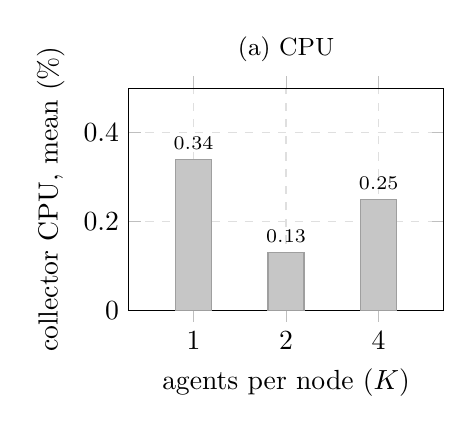
\begin{tikzpicture}
\begin{axis}[
    width=0.46\linewidth, height=4.4cm,
    ybar, bar width=13pt,
    xlabel={agents per node ($K$)}, ylabel={collector CPU, mean (\%)},
    symbolic x coords={1,2,4}, xtick=data,
    ymin=0, ymax=0.5,
    nodes near coords, every node near coord/.append style={font=\scriptsize, text=black},
    grid=major, grid style={dashed,gray!25},
    tick style={draw=gray!50},
    enlarge x limits=0.35,
    title style={font=\small}, title={(a) CPU},
]
\addplot[fill=gray!45, draw=gray!75, mark=none] coordinates {(1,0.34) (2,0.13) (4,0.25)};
\end{axis}
\end{tikzpicture}
\hfill
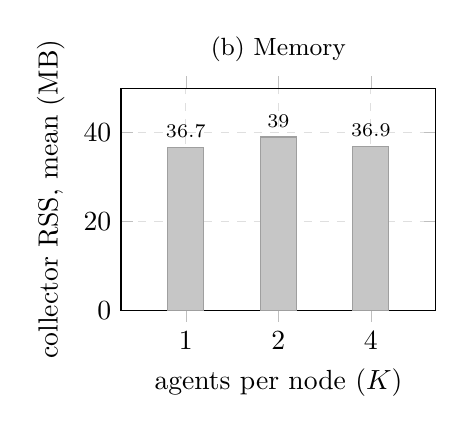
\begin{tikzpicture}
\begin{axis}[
    width=0.46\linewidth, height=4.4cm,
    ybar, bar width=13pt,
    xlabel={agents per node ($K$)}, ylabel={collector RSS, mean (MB)},
    symbolic x coords={1,2,4}, xtick=data,
    ymin=0, ymax=50,
    nodes near coords, every node near coord/.append style={font=\scriptsize, text=black},
    grid=major, grid style={dashed,gray!25},
    tick style={draw=gray!50},
    enlarge x limits=0.35,
    title style={font=\small}, title={(b) Memory},
]
\addplot[fill=gray!45, draw=gray!75, mark=none] coordinates {(1,36.7) (2,39.0) (4,36.9)};
\end{axis}
\end{tikzpicture}

  \caption[Per-node capture load vs.\ agents per node]{Per-node capture load
  as agents per node quadruples, measured on the live 8-node sweep with real
  agents ($K \in \{1,2,4\}$, i.e.\ 8, 16 and 32 agents in total). Both axes
  start at zero, and neither quantity trends: the collector's mean CPU is
  non-monotonic in $K$ (noise around a constant, not growth) and its
  resident memory moves by ${\sim}2$\,MB across the sweep. This is the
  design's prediction (one collector, one keeper and one capture worker
  serve a node regardless of how many agents run on it), so adding agents
  costs the LLM provider, not the capture plane. CPU and memory are drawn on
  separate axes because they share no unit; the transient forward bursts to
  ${\sim}21\%$ are not shown, being spikes rather than sustained load.}
  \label{fig:agents-per-node}
\end{figure}

\section{Functional Validation}
\label{sec:eval-functional}

The system's end-to-end correctness claim, capture through the log store to
every view with real agents on a real cluster (R1, R3, R7), is
validated by an automated harness rather than by demonstration. The
harness brings up the full deployment on a live allocation, runs real
Claude agents (genuine LLM turns; one cross-node MCP delegation
per agent), waits out the drain, restarts the dashboard cold against the
same log store (so everything shown is reconstructed from durable state,
not process memory), and then asserts machine-checkable properties of
every API the dashboard serves: each view is populated with the expected
entities, per-agent metrics are non-zero where turns occurred, and
inter-agent edges exist with correct endpoints. The strictest check is
the cross-plane join: the scenario graph's clicked node resolves to that
agent's conversation with its turns and token counts, exercising the
session-identity contract of \S\ref{sec:design-mapping} end to end.

The harness passes \textbf{28/28} checks on live 4-node and 8-node
ChronoLog clusters. Beyond the pass count, the harness is the regression
suite the design was corrected against: the read-only rule, the archive-first
index read, and the hostname canonicalization of
\S\ref{sec:design-isolation} were each introduced to turn a live-cluster
failure of this harness into a pass, and remain pinned by it.

\section{Case Study: Fault Injection and Localization}
\label{sec:eval-casestudy}

The final question is whether the pieces compose into the cross-layer
diagnosis the thesis promises. The scenario: on a live $M$-node
deployment carrying steady background traffic, the synthetic generator
injects a retry/timeout storm concentrated on one node, alongside a
delegation leg that starts and never completes. The fault is deliberately
of the fail-slow rather than fail-stop kind~\cite{gunawi2018failslow}: the
node stays up, keeps answering, and merely degrades, which is the case a
liveness check cannot see and a population comparison can.

The observed localization path runs one view per operator question. A
Doctor scan returns not hundreds of error rows but a short ranked list:
one incident aggregating the storm (count in the hundreds, blast radius
naming the affected hosts and sessions, root cause and remediation
attached) and one \emph{critical} orphan-call incident for the hung
delegation, invisible in any per-edge view because its signature is an
absence. The fleet heatmap turns ``the fleet looks unhealthy'' into
``it is this machine'': one red cell among ok nodes. The trace
waterfall for the affected scenario charges the bottleneck hop by
self-time, landing on that same node. Clicking the offending agent
opens its conversation, the actual turns, retries and costs behind the
symptom, completing the pivot in two clicks. Re-running the fault
and re-scanning badges the incident \texttt{recurring $\times N$}: the
second occurrence is recognized, not rediscovered. Between them the five
operator questions of \S\ref{sec:problem-scenario} are answered in one
pass over one fault.

\paragraph{Timed comparison.} The path above was then measured as a
controlled exercise on the live 8-node deployment. Faults were injected
by script (a 6-turn identical-prompt 5xx retry storm on one node, twelve
peer-timeout delegations into it, and one delegation leg killed after
its \texttt{start} frame), and a diagnostician answered three questions,
once through the dashboard and once from the raw capture files with
shell tools only, against a verifiable ground truth: \emph{which node is
failing, and with what error}; \emph{which session is retrying, and on
what prompt}; and \emph{which delegation never completed}, named by
caller${\to}$callee and correlation id. The operator was the author, timing each question
from first interaction to stated answer, with every answer checked
against the injected values (including the orphan's correlation id).
Table~\ref{tab:casestudy} reports the result.

\begin{table}[h]
\centering
\small
\begin{tabular}{@{}llrrrl@{}}
\toprule
\textbf{Operator} & \textbf{Interface} & \textbf{Node} &
\textbf{Session} & \textbf{Orphan} & \textbf{Outcome} \\
\midrule
Human, first exposure & dashboard & 35\,s & 17\,s & 20\,s & 3/3 correct (72\,s) \\
Human, second pass    & dashboard & 10\,s & 5\,s  & 5\,s  & 3/3 correct (20\,s) \\
Human, third pass     & dashboard & 5\,s  & 5\,s  & 5\,s  & 3/3 correct (15\,s) \\
Human                 & raw logs  & \multicolumn{3}{c}{abandoned at ${\sim}$5--10\,min} & \textbf{0/3} \\
LLM agent             & raw logs  & \multicolumn{3}{c}{44\,s wall-clock, 4 commands} & 3/3 correct \\
\bottomrule
\end{tabular}
\caption[Timed diagnosis of the injected fault]{Timed diagnosis of the injected fault, $n{=}1$ operator
(first-ever exposure to the task). The three timed columns are the
three questions above, in the order asked. Dashboard trials repeat the same
questions, so passes 2--3 measure a practiced operator. The raw-log
attempt ran \emph{after} the dashboard trials (answer leakage, if
any, favored the raw-log path) and still produced no answers: the
operator could not establish a starting point in the JSONL directories.
The supplementary row is a fresh LLM agent given only the three
questions and the data directories (no ground truth, shell text tools
only); machine wall-clock is not comparable to human minutes and is
reported for what it demonstrates about the \emph{data}, not the
operator.}
\label{tab:casestudy}
\end{table}

Two findings, one expected and one not (the second previewed in
\S\ref{sec:bg-sota-gap}). The expected one: a first-time operator
produced a complete, verified diagnosis through the dashboard in
\textbf{72 seconds}, yet could not answer \emph{any} of the three
questions from the raw files, abandoning after five to ten minutes
without a foothold. The dashboard run included recovering from one
wrong pick on the orphan question: the twelve errored-but-completed delegations
rendered adjacent to the true orphan, and the correlation-id check
caught the confusion. The unexpected one: the LLM-agent baseline
answered all three questions from the raw JSONL in 44 seconds and four
shell commands, finding the orphan by counting correlation-id
occurrences, the very question the protocol predicted would time out
under \texttt{grep}. Together they sharpen what this chapter can
claim: the capture layer's raw data is \emph{sufficient} for
complete diagnosis, but it is not \emph{accessible}: extracting the
answer requires either expertise the on-call operator does not have or
tooling that encodes it. The dashboard is that encoding: it substitutes
for operator expertise, not for data.

The caveats are plain: one operator, one injected incident on a small
scenario corpus, and a
UI defect surfaced by the stumble on the orphan question (never-completed delegations
rendered indistinguishably from completed ones). That defect was fixed
following the study. Open delegations now carry a dedicated visual
class (amber, dashed, badged \emph{never completed}) across the
scenario graph, the edge detail panel, and the trace waterfall, and
hung flows outrank errors in edge selection; the pathology that cost
the operator their one wrong pick is now the most visually distinct
element on screen (Figure~\ref{fig:ui-orphan}).

\section{Discussion and Limitations}
\label{sec:eval-limitations}

\paragraph{Hot store locality.} The hot store and live bus live with the
dashboard process; they are not replicated. A dashboard failure loses no
data (the log is authoritative; the hot view rebuilds from backlog and,
after the drain, from ChronoLog) but interrupts live observation:
acceptable for an operator tool, but a real asymmetry with the
replicated cold path.

\paragraph{Two properties of the deployment, not of this design.} The
measured 20--30\,s cold-path latency follows from the ChronoLog
deployment's chunking and acceptance-window configuration rather than from
anything this system does; the design works around
it rather than removing it, and a deployment with tighter chunking would
narrow the hot/cold gap without changing the architecture.

A second property surfaced during the evaluation itself. In the
deployments measured here, playback responses from the player were not
observed to reach the dashboard process's receiver service: the requests
appear in the player's log, no transfer toward that endpoint completed
during these runs, and an otherwise-identical receiver hosted in the
capture process did receive them. The effect is that a live replay issued
from the dashboard ran to the ${\sim}180$\,s query timeout while holding
the client lock. This thesis does not diagnose the cause and does not
claim one; the observation is scoped to the version, configuration and
client binding deployed here, and is reported so that the workaround it
motivated is reproducible rather than unexplained. That workaround was to
generalize the archive-first
rule: with \texttt{CHRONOLOG\_ARCHIVE\_FIRST} set, the dashboard and
capture worker serve all replay reads from the grapher's archive and
never ask the player, bounding worst-case staleness at the measured
drain window. It is the right trade under the behavior observed, but it
leaves the live-replay path unused, and a deployment in which that path
returns would recover it.

\paragraph{Diagnosis coverage.} The heuristic diagnoser is
first-match-wins over a hand-built rule set: specific on the failure
classes it encodes, and explicitly low-confidence outside them. It
explains known pathologies; it does not discover novel ones. The
signature scheme can also split one logical failure into two incidents if
its message text varies beyond what normalization strips.

\paragraph{Evaluation scale.} Live validation ran at $M \in \{4, 8\}$
with real agents (the allocation sizes available), while the
100+-node claims rest on the rollup complexity argument and seeded
fleet-scale data rather than a live fleet of that size. The p95 fold of
\S\ref{sec:analytics-fleet} is upper-biased by construction, and
inferred (parentless) traces rely on time nesting, which can
mis-parent overlapping concurrent delegations between the same pair of
agents; explicit parent propagation removes the ambiguity where the
instrumentation provides it.

\medskip

Taken together, the six questions this chapter opened with have
quantitative answers: capture is statistically invisible to the agent,
live views run three orders of magnitude ahead of the durable drain,
detection is exact on ground truth, the fleet reads scale as designed,
the stack survives real agents on real clusters, and the path from
symptom to cause takes an untrained operator seventy-two seconds. What
these answers add up to, and what they cost, is the subject of the
concluding chapter.
